
\TuscConcept{SLIM} employs a simple distributed and randomized TDMA scheme. 
Using \TuscConcept{SLIM}, each node continuously listen to the channel for any transmission that it can decode unless it transmits a message. 
Each node individually selects random slots to transmit its messages.
In the case of two or more nodes selecting the same slot, unless one of the transitions capture receivers with a high SINR, the transmissions results in a collision preventing successful reception of all colliding transmissions.

As depicted in \cref{Fig:WaveformModules}, SLIM waveform consists of:
\begin{itemize}
\item a channel that consists of a propagation loss model and and propagation delay model,
\item a phy layer that consists of an interference helper,
\item a net device that implement MAC layer and an interface for the interaction with upper layers.
\end{itemize}

\begin{figure}[h]
 \centering
 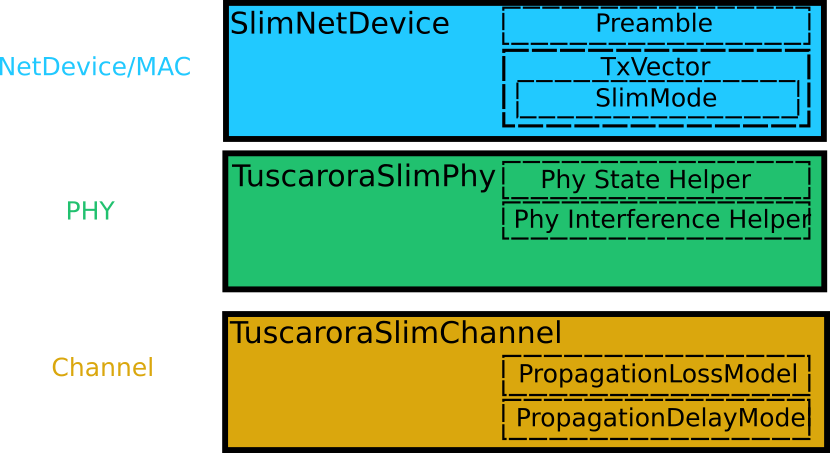
\includegraphics[width=0.9\linewidth]{figures/SLIM_Modules}
 \caption{Waveform modules}
 \label{Fig:WaveformModules}
\end{figure}

\section{Adapting SLIM Waveform}

SLIM waveform can be adapted for a large class of waveforms whose characteristics under constant SINR are known apriori. 

First an error function is derived from SlimModeError which simply implements a \CPPFuncName{GetBER(double sinr)} function. An example of this is given in \CPPClassName{TuscaroraDsssDbpskModeError}. 

In the next stage, the user creates the \CPPClassName{SlimMode} objects with unique names and setting their parameters. 
The input variables that should be specified for each mode is listed in \cref{table:SlimModeTable} along with their defaults.

 \begin{longtable}{ | c | c | c |}

\caption{Attributes of SlimMode}\label{table:SlimModeTable}	\\
 
     \hline
  \textbf{Attribute} & \textbf{Short Description} & \textbf{Default Value} \\ \hline
 
     
    
 UniqueName & \parbox[][][t]{7cm}{\vspace{6pt}\raggedright A unique name for the mode\vspace{6pt}} & 
                   "UNINITIALIZEDMODE" \\ \hline 

 Bandwidth &  \parbox[][][t]{7cm}{\vspace{6pt}\raggedright The bandwidth(Hz) of the signal being modeled.\vspace{6pt}} & 
                   20000 \\ \hline 
                   
 Tpb & \parbox{7cm}{\vspace{6pt}\raggedright Time it takes to transmit one bit of information. Only needed for modes specifying payload.\vspace{6pt}} & 
                   1000ns \\ \hline 	
                   
Duration & \parbox{7cm}{\vspace{6pt}\raggedright Total time it takes to transmit the section. Only needed for fixed length sections of a packet. Calculated internally for payload.\vspace{6pt}} & 
              1000ns\\ \hline            
  
FecF & \parbox{7cm}{\vspace{6pt}\raggedright The fraction of bits that the FEC can correct. A double value.\vspace{6pt}} & 
                  0.0\\ \hline 	
                                   
ErrorModPtr & \parbox{7cm}{\vspace{6pt}\raggedright Pointer to the SlimModeError object implementing SINR vs. BER characteristics. The default is of type TuscaroraDsssDbpskModeError.\vspace{6pt}} & 
               NULL\\ \hline       
               



%m\_noiseFigure & \parbox{5cm}{\centering Loss  } & 
%              MicroSeconds(0)\\ \hline               

       							  		
	   
 \end{longtable}   


Next, \CPPClassName{SlimTxVector} objects that represent the transmission characteristics of packets are created. This object holds a vector of previously created \CPPClassName{SlimMode} objects each representing a part of the packet such as preamble or a specific level header. All of the modes have fixed sizes except for the payload whose size is the determined at the time of the transmission. The position of the payload relative to other parts of the packet in the vector is explicitly specified using \CPPFuncName{SetPayloadModePosition(uint8\_t k)}.

 \begin{longtable}{ | c | c | c |}

\caption{Attributes of SlimTxVector}\label{table:SlimTxVectorTable}	\\
 
     \hline
  \textbf{Attribute} & \textbf{Short Description} & \textbf{Default Value} \\ \hline
 
     
    
 UniqueName & \parbox[][][t]{5cm}{\vspace{6pt}\raggedright A string containing a uniqueName of the TxVector. Used for comparison purposes.\vspace{6pt}} & 
                   "UNINITIALIZEDTXVECTOR" \\ \hline 

 PayloadModePosition &  \parbox[][][t]{5cm}{\vspace{6pt}\raggedright The index of the section containing the payload. \vspace{6pt}} & 
                   0 \\ \hline 
                   



%m\_noiseFigure & \parbox{5cm}{\centering Loss  } & 
%              MicroSeconds(0)\\ \hline               

       							  		
	   
 \end{longtable}   


Each \CPPClassName{TuscaroraSlimPhy} object holds a list of \CPPClassName{SlimTxVector} objects. This lists determines the capabilities of the PHY to transmit/receive packets encoded with the underlying transmission characteristics. 

In the final stage, \CPPClassName{SlimTxVector} objects created in the previous stage is added to this list. Along with these characteristics a channel number is defined for the PHY. This can be changed at any instant and only phy object operating on the same channel are able to communicate with each other. 

\section{SlimNetDevice}

The \CPPClassName{SlimNetDevice} is the top layer providing an interface to the upper layers using the waveform as a communication device.
\CPPClassName{SlimNetDevice} has various attributes that can be customized on the fly. These are summarized in \cref{table:SlimNetDeviceTableofAttributes}.

%\begin{description}
% \item[TxMode] The i'th TxMode in the list of allowed txmodes by the attached phy layer. The default value of this attribute is 0, making \CPPClassName{SlimNetDevice} use the first txmodes in the list of tx modes offered by the PHY layer.  
%
% \item[ContentionWindowSize] The window size among which to select the next tx slot. The default value of this attribute is 10.
%
% \item[SlotDuration] The size of each slot(in ns3::Time type). The default value of this attribute is 1ms.
%
% \item[TxQueue] A queue to use as the transmit queue in the device. The default value queue used by the device is a DropTailQueue. 
%\end{description}
\begin{longtable}{ | c | c | c |}

\caption{Attributes of TuscaroraSlimNetDevice}\label{table:SlimNetDeviceTableofAttributes}	\\
 
     \hline
  \textbf{Attribute} & \textbf{Short Description} & \textbf{Default Value} \\ \hline
 

 TxVectorIndex &  \parbox[][][t]{6.5cm}{\vspace{6pt}\raggedright The index of the SlimTxVector to be used for transmitting packets in the list of supported SlimTxVectors of the attached phy layer.\vspace{6pt}} &  0 \\ \hline 

 ContentionWindowSize &  \parbox[][][t]{6.5cm}{\vspace{6pt}\raggedright Average number of slots in between two selected transmission slots.\vspace{6pt}}  & 10 \\ \hline 

 SlotDuration &  \parbox[][][t]{6.5cm}{\vspace{6pt}\raggedright The size of each slot(in ns3::Time type).\vspace{6pt}} & 1ms \\ \hline 
 
				   
 TxQueue &  \parbox[][][t]{6.5cm}{\vspace{6pt}\raggedright The pointer to a queue object used as the transmit queue in the device.\vspace{6pt}}  & DropTailQueue \\ \hline 
			   			   
				   
	   
 \end{longtable}   



Upper layers pass the packets using \CPPClassName{SlimNetDevice}'s \CPPFuncName{Send} routine. These packet gets queued up and are transferred to the \CPPClassName{TuscaroraSlimPhy} one by one during the chosen transmission slots. Outgoing packages are stored in a customizable queue. The default queue is of \TuscConcept{DropTailQueue} type and can be customized using any standard queue object through the attribute \TuscConcept{TxQueue} of the \TuscConcept{slim-net-device}.

Multiple packets can be transmitted in a given transmission slot depending on the size of the packets. 
At the end of each transmission, 
if there are remaining packets in the \CPPVarName{TxQueue} and
the time it takes to transmit the next packet is less than the remaining time of the slot, \CPPClassName{SlimNetDevice} starts the transmission of the next packet. 
Otherwise, \CPPClassName{SlimNetDevice} waits for the next transmission slot. 

The slot timing and boundaries are synchronous but the slot selection algorithm is distributed and independent. The next transmission slot is selected randomly from a range of [1-\CPPVarName{ContentionWindowSize}] slots. The max limit of this range determines the average frequency of slot selection and can be adjusted on the fly using the attribute \CPPVarName{ContentionWindowSize}. The default value of \CPPVarName{ContentionWindowSize} is ten slots. 

On the receiving side, \CPPClassName{SlimNetDevice} checks the destination field of the packets and drops the packets that are not destined for the node. In addition to this, \CPPClassName{SlimNetDevice} offers a promiscuous packet sniffer and callback. If this mode is used, all packets are passed to the chosen callback regardless of the destination.  

\section{TuscaroraSlimPhy}

The \CPPClassName{TuscaroraSlimPhy} implements the PHY layer functions for the \TuscConcept{SLIM} waveform. \CPPClassName{TuscaroraSlimPhy}'s main duties are: 
(i) keeping the state of the physical layer, 
(ii) setting the modulation type for the packets and calculating their transmission duration, 
(iii) keeping track of the interference level using the \CPPClassName{SlimInterferenceHelper}, and 
(iv) deciding on whether a packet is successfully received or had unrecoverable errors using \CPPClassName{SlimInterferenceHelper} and the error characteristics of the \CPPClassName{SlimMode}s making up the packet.
\CPPClassName{TuscaroraSlimPhy} has various attributes that can be customized on the fly. These are summarized in \cref{table:SlimPhyTableofAttributes}.





On the sender side, 
%\CPPClassName{TuscaroraSlimPhy} receives packets from the net-device using \CPPClassName{TuscaroraSlimPhy}'s \CPPFuncName{SendPacket} routine.
\CPPClassName{SlimNetDevice} create a \CPPClassName{SlimTxVector} setting packet properties such as the modulation class and FEC characteristics and set the transmit power level and the payload size. 
Then, the packet is passed down using \CPPClassName{TuscaroraSlimPhy}'s \CPPFuncName{SendPacket} routine that further sends the packet down to the channel and schedules the end of the transmission for state changes. 
All devices operating on the same channel number as the transmitting device are invoke for packet reception. The channel also calculates the power level at each receiver using the chosen \CPPClassName{PropagationLossModel}. The antenna gains relative to the isotropic antenna are calculated based on the \CPPClassName{AntennaModel} and the relative angle between the devices and added to the received power.


 \begin{longtable}{ | c | c | c |}

\caption{Attributes of TuscaroraSlimPhy}\label{table:SlimPhyTableofAttributes}	\\
 
     \hline
  \textbf{Attribute} & \textbf{Short Description} & \textbf{Default Value} \\ \hline
 
     
    
 EnergyDetectionThreshold & \parbox[][][t]{5cm}{\vspace{6pt}\raggedright The energy of a received signal should be higher than 
                   this threshold (dbm) to allow the PHY layer to detect the signal.} & 
                   -96.0 \\ \hline 

 TxGain & \parbox[][][t]{5cm}{\vspace{6pt}\raggedright Transmission gain (dB).} & 
                   1.0 \\ \hline 

 RxGain & \parbox[][][t]{5cm}{\vspace{6pt}\raggedright Reception gain (dB).} & 
                   1.0 \\ \hline 

 TxPowerLevels & \parbox[][][t]{5cm}{\vspace{6pt}\raggedright Number of transmission power levels available between 
                   TxPowerStart and TxPowerEnd included.} & 
                   1 \\ \hline 

 TxPowerEnd & \parbox[][][t]{5cm}{\vspace{6pt}\raggedright Maximum available transmission level (dbm).} & 
                   16.0206 \\ \hline 

 TxPowerStart & \parbox[][][t]{5cm}{\vspace{6pt}\raggedright Minimum available transmission level (dbm).} & 
                   16.0206 \\ \hline 

 RxNoiseFigure & \parbox[][][t]{5cm}{\vspace{6pt}\raggedright Loss (dB) in the signal to noise ratio due to non-idealities in the receiver.} & 
                   0 \\ \hline 

 StateHelperPtr & \parbox[][][t]{5cm}{\vspace{6pt}\raggedright The pointer to the helper class object that keeps the state of the phy layer} & 
                   PointerValue () \\ \hline 

 ChannelSwitchDelay & \parbox[][][t]{5cm}{\vspace{6pt}\raggedright Time it takes to switch channels.} & 
                   250000ns \\ \hline 

 ChannelNumber & \parbox[][][t]{5cm}{\vspace{6pt}\raggedright Channel number among multiple orthogonal channels.}
 %Channel center frequency = Channel starting frequency + 5 MHz * nch} & 
                  & 1 \\ \hline 

 Frequency & \parbox[][][t]{5cm}{\vspace{6pt}\raggedright The central operating frequency.} & 
                   2407 \\ \hline 

 AntennaPtr & \parbox[][][t]{5cm}{\vspace{6pt}\raggedright The pointer pointing to the associated antenna object.} & 
                  IsotropicAntennaModel \\ \hline 

% Transmitters & \parbox[][][t]{5cm}{\vspace{6pt}\raggedright The number of transmitters.} & 
%                   UintegerValue (1) \\ \hline 
%
% Receivers & \parbox[][][t]{5cm}{\vspace{6pt}\raggedright The number of receivers.} & 
%                   UintegerValue (1) \\ \hline 
%
% ShortGuardEnabled & \parbox[][][t]{5cm}{\vspace{6pt}\raggedright Whether or not short guard interval is enabled.} & 
%                   BooleanValue (false) \\ \hline 
%
% LdpcEnabled & \parbox[][][t]{5cm}{\vspace{6pt}\raggedright Whether or not LDPC is enabled.} & 
%                   BooleanValue (false) \\ \hline 
%
% STBCEnabled & \parbox[][][t]{5cm}{\vspace{6pt}\raggedright Whether or not STBC is enabled.} & 
%                   BooleanValue (false) \\ \hline 
%
% GreenfieldEnabled & \parbox[][][t]{5cm}{\vspace{6pt}\raggedright Whether or not STBC is enabled.} & 
%                   BooleanValue (false) \\ \hline 
%
% ChannelBonding & \parbox[][][t]{5cm}{\vspace{6pt}\raggedright Whether 20MHz or 40MHz.} & 
%                   BooleanValue (false) \\ \hline 
%
% CenterFrequency & \parbox[][][t]{5cm}{\vspace{6pt}\raggedright The center frequency of the channel} & 
%				   DoubleValue (2407) \\ \hline 
%
% RateDefinitions & \parbox[][][t]{5cm}{\vspace{6pt}\raggedright The objects that hold rates supported} & 
%				   PointerValue () \\ \hline 

 
				   

			   
				   
				   
	   
 \end{longtable}   


On the reception side, \CPPClassName{TuscaroraSlimPhy} receives packets from the channel using \CPPFuncName{StartReceivePacket} function. The average reception power of all packets are recorded using the \CPPClassName{SlimInterferenceHelper} in a linked list together with their start and ending time instances. 
Although all packets are considered as a possible interferer, only for packets that have a larger power than \CPPVarName{EnergyDetectionThreshold} are considered for reception and an \CPPFuncName{EndReceive} event is scheduled. \CPPFuncName{EndReceive} function determines whether the reception was indeed successful by considering the modulation characteristics specified by the associated \CPPClassName{SlimTxVector}.


In calculating the packet error rate, \CPPClassName{SlimInterferenceHelper} takes into account the cumulative list of interference events throughout the packet duration as kept by the and the particular modulation and FEC scheme employed. 

Each packet consists of sections with possibly different error characteristics due to the underlying modulation and FEC characteristics. For instance, for many waveforms the preamble section is more vulnerable to interference compared to the rest of the packet. Similarly, due to compatibility issues, certain headers might have different characteristics than the payload. These characteristics are abstracted in a \CPPClassName{SlimMode}. 

The \CPPClassName{SlimModeError} for each \CPPClassName{SlimMode} implement an error function describing the relationship between the SINR and the BER characteristics excluding the FEC. Total number of errors in the section is calculated based on the \CPPClassName{SlimModeError} under varying SINR. This number is compared with the total number of errors that can be corrected by the FEC to determine whether packet can be successfully received or not. 

The defaults in the \CPPClassName{SlimNetDevice} uses a single modulation and FEC rate for the entire packet. Since the packet consists of a single section, the packet success rate entirely depends on the random number of bit errors in the packet and error correction capabilities of the FEC algorithm. 

\section{TuscaroraSlimChannel}

The \CPPClassName{TuscaroraSlimChannel} object connects the \CPPClassName{TuscaroraSlimPhy} objects of various nodes to each other. Its main duties are: (i) calculating the received power levels on each node using the propagation loss model, (ii) calculating the time instance with which the packet reaches to the nodes using the propagation delay model, (iii) initiating reception on each node's phy layer. 
\CPPClassName{TuscaroraSlimChannel} has various attributes that can be customized on the fly. These are summarized in \cref{table:TuscaroraSlimChannelTableofAttributes}.

 \begin{longtable}{ | c | c | c |}

\caption{Attributes of TuscaroraSlimChannel}\label{table:TuscaroraSlimChannelTableofAttributes}	\\
 
     \hline
  \textbf{Attribute} & \textbf{Short Description} & \textbf{Default Value} \\ \hline
 
 PropagationLossModel & \parbox{6cm}{\centering A pointer to the propagation loss model attached to this channel.} & 
                   PointerValue () \\ \hline 

 PropagationDelayModel & \parbox{6cm}{\centering A pointer to the propagation delay model attached to this channel.} & 
                   PointerValue () \\ \hline 
			   
				   
				   
	   
 \end{longtable}   


 